
\chapter{Comparison with existing technologies}
\label{chapter:comparison}

A detailed description is provided in this section concerning the state of the art technologies existing nowadays in the
market. Current Integration technologies available today are based on the SOA and REST architectural styles, with Web Services
and REST on HTTP as the most used implementations. This section also gives information about tools that we will use in our
solution.


%%%%%%%%%%%%%%%%%%%%%%%%%%%%%%%%%%%%%%%%%%%%%%%%%%%%%%%%%%%%%%%%%%%%%%%%
\section{Web Services}
\label{section:webservices}

Web services allow you to use two different machines or two different pieces of code that talk each other. Two different
applications can talk to each other over the network. They can call methods of each other over the network by using web
service technology. The other advantage of using web services is actually it is a standard technology because it is not
really specific to java or any other language. You can write web services all other technologies. For example you can write
web service with Java, .Net, Python, C++ or others. The best part of web service standard what is called as Interoperability
that  is a property of a product or system, whose interfaces are completely understood, to work with other products or
systems, present or future, without any restricted access or implementation\citep{interoperability:2016:Online}.\\

\begin{figure}[!htb]
  \centering
  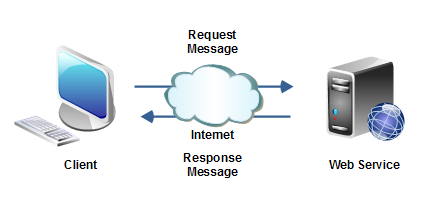
\includegraphics[width=0.5\textwidth]{Figures/web-service-message-formats-1.png}
  \caption[Simple Web Service Architecture.]{Simple Web Service Architecture.}
  \label{fig:webservice}
\end{figure}

For example let’s say you have written web service in Java, let’s say you have another web service that written in .Net so what
the web service technology allows you to do is Java can call .Net web service and .Net web service can also call Java web
service and it just doesn’t have to be web service let’s say you have another application written in C++, so you can actually
have C++ app that call java web service or .Net web service. You can actually have different applications written in different
technologies that communicate with each other during execution time and they can call each other. This actually let us do is
you can actually pick and choose technologies that you want to use let’s say you have set of business web services that are
implemented in .Net and your java application can use them.\\

Web Services are exposed to the Internet for programmatic access. They are online APIs that you can call from your code.
When you want to call any API that written by someone else to your java code, you basically add jar or classes to your class
path and executions are done inside of machine or single environment. In the case of web services however you have different
pieces of code deployed over different machines and they call methods of each other over the network. For example, you must
have seen that different apps or games, which can post to your Facebook wall even these games, not designed by Facebook.
So you ask that how they can do that or how they can post to a wall of completely different system or application. Basically
they do this by calling online APIs. Companies like Facebook or Twitter publish web services that let other developers call
them from their code, so other application developers can actually write code to consume these services and they can post
things on Facebook or Twitter. They can read or access data from Facebook or Twitter using the APIs of the web services that
Facebook or Twitter has provided.\\

Web services are similar to web pages. For example Twitter has web side URL as “www.twitter.com“ when you access this URL on
your browser you get an HTML response that let you read and write tweets. They have HTML elements for data and also CSS files
for styling, this is because web pages that you see are made human conception. They know that there is actually human is behind
of browser on a laptop or devices who was reading these tweets, so they want to make sure about its format properly, so it is easy to access and read.
Twitter has also other URL as “api.twitter.com“ that does a lot of same things as “www.twitter.com“ does, but it behaves a bit
differently for instance this API gives you response which doesn’t have HTML or CSS code. It contains data but it is xml or json format and there are specific URLs for different operations this is what the developers can use from their code to read or write to twitter, so this data is actually very easy for parsing and converting then using in their objects and their code for developers. In this case there is no need HTML and CSS files.\\
There are primarily two different types of web services. One of these types called as  Simple Object Access Protocol (SOAP) web
service and another type called as REpresentational State Transfer(REST) web service. SOAP is older of these two and REST is newer entry to web services world, but both of them are used popular.
Next chapter will be focusing on SOAP and REST web services.

%%%%%%%%%%%%%%%%%%%%%%%%%%%%%%%%%%%%%%%%%%%%%%%%%%%%%%%%%%%%%%%%%%%%%%%%
\section{SOAP Web Services}
\label{section:soa}

Simple Object Access Protocol, or SOAP as it was the first attempt to standardize a web service interface. It is based on
sending an XML message to a service, in a specific format, and receiving an XML response in another specific format.
The message can be sent across different transports, including HTTP, FTP, SMTP, and more. The specification does not
dictate the transport over which the message should be sent, but most implementations send the XML message over HTTP.\\

I will try to explain shortly SOAP web service by an example. Let’s start an example with java application. Let’s say we have
implementation class and I want to share this implementation class with other developer projects. How I would share this with a
consumer class. The best way to share this implementation class would be to contract it with an interface and other consumers
would consume this class through this interface. They would call implementation through interface so they get contract and they
get the methods, arguments, written types through interface. They actually call the methods of implementation class, so how this
works in case of web service, let’s say I have web service implementation and I want to share details of this web service to
consumers. Is it works with an interface? Probably it will not work because as we discussed before you don’t know what technology
is consuming it. It might be .Net application or C++ application, so if you have a java web service you might want to give some
kind of information that its consumer respects to that technology and that can actually consume. Let’s say consumer is .Net and if I give this .Net
application a java interface then most probably it will not work because they are different technologies, so the technology
that we are going to share with web service consumer has to be technology independent. It should be something that any
application or any technology can understand so creators of SOAP web service talked about that problem and what to give format
understandable by all technology with all consumers and decided with XML. So what we do is in case of web service, we
actually share that contract as an XML document. This XML document is actually called as WSDL.\\

WSDL document contains the contract to web service and so that’s are the things you have to do when you create the web
service and you share WSDL document of that web service to the consumers, so this is not something you would have to do
it manually. You would do it manually but there are tools which generate WSDL for the web service but it is something that
you need to share this WSDL to consumers and it is a XML document, so it respective whatever application because applications
such as .Net, C++ or Java can all parse this XML and get to know about service information and typically the content of
this WSDL is kind of similar to an interface content. It has operations, arguments and types  to return that consumer
applications will have idea what to call and how to call.\\

\begin{figure}[!htb]
  \centering
  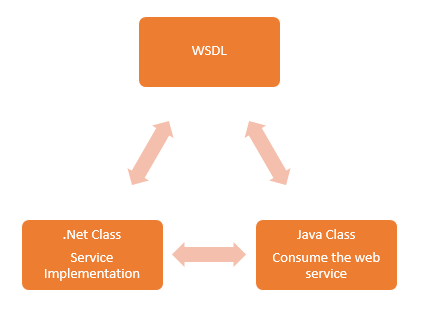
\includegraphics[width=0.5\textwidth]{Figures/WSDL.png}
  \caption[WSDL file.]{WSDL file.}
  \label{fig:wsdl}
\end{figure}

The new question is that how this exchange happens, how you actually send this information, let’s say you have a method in
your java application and input argument is a string so you have a java string with you and you need to send to web service
and let’s say output return type is a list, so how you get this information because that could be .Net application and string
in java obviously different from string in .Net. How do you exchange this between client app and web service?  When you exchange
information input argument or return type you need to exchange it in the format that all different technologies can understand
what you are passing and it should be able to send return type back in language that all these technologies can understand.
Again this format is XML. When you are sending any information across the network from a client to the web services and
return type back to the client, the data has to be in XML format. You are not really sending java string or a list. So it
has to be language natural format which is XML. There is specification about how you need to send all these different input
type and output argument basically any type needs to be send specific XML format.\\

It is a protocol that is a way in which both sender and receiver and this XML is called SOAP.
It is a way in which these different technologies can access objects can access data it supposedly simple so that a part
of the name is called simple object access protocol. So with this protocol all different technologies written in different
languages can kind of understand what they all taking about.\\

\begin{figure}[!htb]
  \centering
  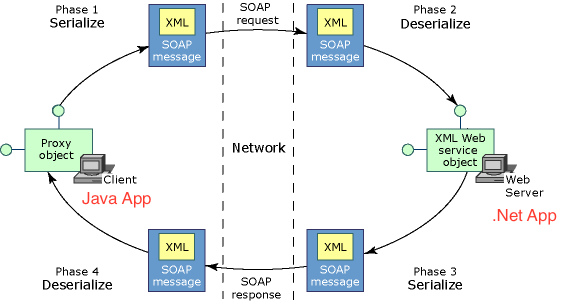
\includegraphics[width=0.8\textwidth]{Figures/soap.png}
  \caption[SOAP.]{SOAP.}
  \label{fig:wsdl}
\end{figure}

Now we know what is the mechanism we know what need to be send and we know how to send which is using SOAP protocol
but who does conversion? So for example you have your string object or complex object, so how do you convert it from java
object to a soap message? The conversion is actually done with intermedia class so this class takes care of converting all
your objects into a SOAP message. The whole method calls itself is actually done by SEI(Service Endpoint Interface). The SEI access interface to your
web service endpoint so you have an interface at your client app to the service endpoint which translate all web service
call to a SOAP message and then it makes sure that the other things is able to understand this message. So we don’t have to
write this class and all the conversion ourselves. We can have it automatically generated for us. When you are making a web
service call you don’t worry about where the web service is. When you need to call, all you need to do is have this endpoint
interface and good thing about this service endpoint that you can actually have an interface that specific to what you are
developing. When you have a java application you will have a specific SEI for java application and it knows to convert java
objects to SOAP message. Let’s say your .Net application calling the same web service so you will have SEI for .NET that know
to convert .Net objects to SOAP message.\\

%%%%%%%%%%%%%%%%%%%%%%%%%%%%%%%%%%%%%%%%%%%%%%%%%%%%%%%%%%%%%%%%%%%%%%%%
\section{REST Web Services}
\label{section:rest}

Quest for the optimal solution...


% ----------------------------------------------------------------------
\subsection{Figures}
\label{subsection:figures}

Insert your section material and possibly a few figures...

Make sure all figures presented are referenced in the text!


% ----------------------------------------------------------------------
\subsubsection{Images}
\label{subsection:images}

\begin{figure}[!htb]
  \centering
  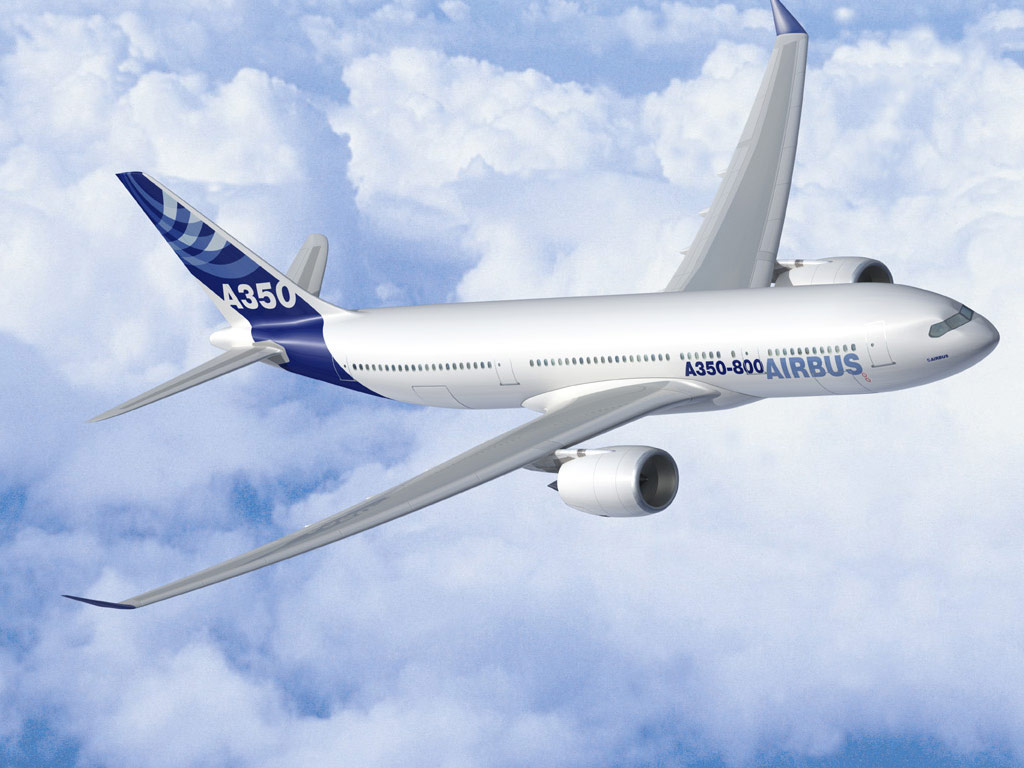
\includegraphics[width=0.25\textwidth]{Figures/Airbus_A350.jpg}
  \caption[Caption for figure in TOC.]{Caption for figure.}
  \label{fig:airbus1}
\end{figure}

\begin{figure}[!htb]
  \begin{subfigmatrix}{2}
    \subfigure[Airbus A320]{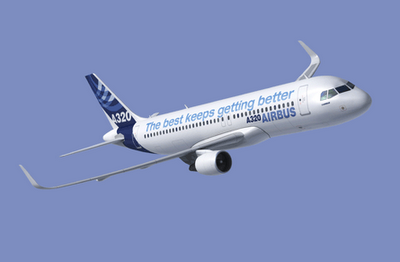
\includegraphics[width=0.49\linewidth]{Figures/Airbus_A320_sharklets.png}}
    \subfigure[Bombardier CRJ200]{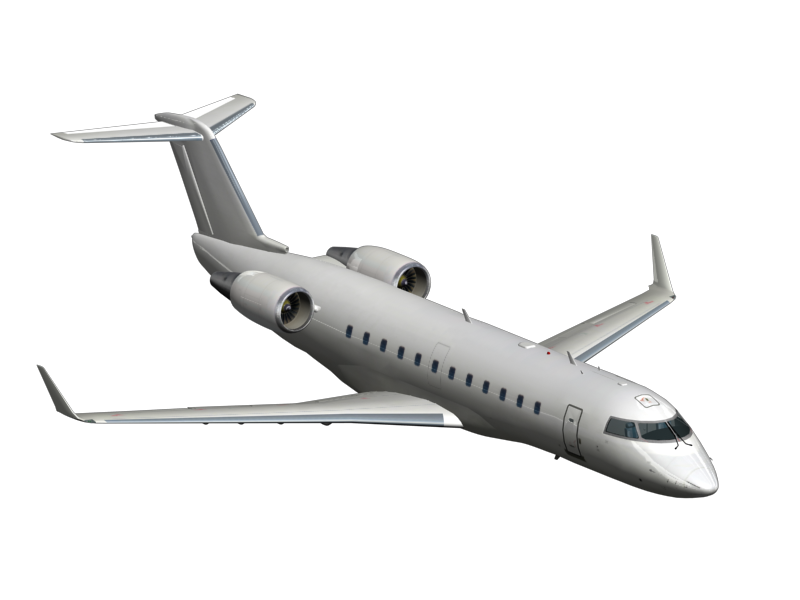
\includegraphics[width=0.49\linewidth]{Figures/Bombardier_CRJ200.png}}
  \end{subfigmatrix}
  \caption{Some aircrafts.}
  \label{fig:aircrafts}
\end{figure}

Make reference to Figures \ref{fig:airbus1} and \ref{fig:aircrafts}.

By default, the supported file types are {\it .png,.pdf,.jpg,.mps,.jpeg,.PNG,.PDF,.JPG,.JPEG}.

See \url{http://mactex-wiki.tug.org/wiki/index.php/Graphics_inclusion} for adding support to other extensions.


% ----------------------------------------------------------------------
\subsubsection{Drawings}
\label{subsection:drawings}

Insert your subsection material and for instance a few drawings...

The schematic illustrated in Fig.~\ref{fig:algorithm} can represent some sort of algorithm.

\begin{figure}[!htb]
  \centering
  \scriptsize
%  \footnotesize
%  \small
  \setlength{\unitlength}{0.9cm}
  \begin{picture}(8.5,6)
    \linethickness{0.3mm}

    \put(3,6){\vector(0,-1){1}}
    \put(3.5,5.4){$\bf \alpha$}
    \put(3,4.5){\oval(6,1){}}
    %\put(0,4){\framebox(6,1){}}
    \put(0.3,4.4){Grid Generation: \quad ${\bf x} = {\bf x}\left({\bf \alpha}\right)$}

    \put(3,4){\vector(0,-1){1}}
    \put(3.5,3.4){$\bf x$}
    \put(3,2.5){\oval(6,1){}}
    %\put(0,2){\framebox(6,1){}}
    \put(0.3,2.4){Flow Solver: \quad ${\cal R}\left({\bf x},{\bf q}\left({\bf x}\right)\right) = 0$}

    \put(6.0,2.5){\vector(1,0){1}}
    \put(6.4,3){$Y_1$}

    \put(3,2){\vector(0,-1){1}}
    \put(3.5,1.4){$\bf q$}
    \put(3,0.5){\oval(6,1){}}
    %\put(0,0){\framebox(6,1){}}
    \put(0.3,0.4){Structural Solver: \quad ${\cal M}\left({\bf x},{\bf q}\left({\bf x}\right)\right) = 0$}

    \put(6.0,0.5){\vector(1,0){1}}
    \put(6.4,1){$Y_2$}

    %\put(7.8,2.5){\oval(1.6,5){}}
    \put(7.0,0){\framebox(1.6,5){}}
    \put(7.1,2.5){Optimizer}
    \put(7.8,5){\line(0,1){1}}
    \put(7.8,6){\line(-1,0){4.8}}
  \end{picture}
  \caption{Schematic of some algorithm.}
  \label{fig:algorithm}
\end{figure}


% ----------------------------------------------------------------------
\subsection{Equations}
\label{subsection:equations}

Equations can be inserted in different ways.

The simplest way is in a separate line like this

\begin{equation}
  \frac{{\rm d} q_{ijk}}{{\rm d} t} + {\cal R}_{ijk}({\bf q}) = 0 \,.
\label{eq:ode}
\end{equation}

If the equation is to be embedded in the text. One can do it like this ${\partial {\cal R}}/{\partial {\bf q}}=0$.

It may also be split in different lines like this

\begin{eqnarray}
  {\rm Minimize}   && Y({\bf \alpha},{\bf q}({\bf \alpha}))            \nonumber           \\
  {\rm w.r.t.}     && {\bf \alpha} \,,                                 \label{eq:minimize} \\
  {\rm subject~to} && {\cal R}({\bf \alpha},{\bf q}({\bf \alpha})) = 0 \nonumber           \\
                   &&       C ({\bf \alpha},{\bf q}({\bf \alpha})) = 0 \,. \nonumber
\end{eqnarray}

It is also possible to use subequations. Equations~\ref{eq:continuity}, \ref{eq:momentum} and \ref{eq:energy} form the Naver--Stokes equations~\ref{eq:NavierStokes}.

\begin{subequations}
    \begin{equation}
    \frac{\partial \rho}{\partial t} + \frac{\partial}{\partial x_j}\left( \rho u_j \right) = 0 \,,
    \label{eq:continuity}
    \end{equation}
    \begin{equation}
    \frac{\partial}{\partial t}\left( \rho u_i \right) + \frac{\partial}{\partial x_j} \left( \rho u_i u_j + p \delta_{ij} - \tau_{ji} \right) = 0, \quad i=1,2,3 \,,
    \label{eq:momentum}
    \end{equation}
    \begin{equation}
        \frac{\partial}{\partial t}\left( \rho E \right) + \frac{\partial}{\partial x_j} \left( \rho E u_j + p u_j - u_i \tau_{ij} + q_j \right) = 0 \,.
    \label{eq:energy}
    \end{equation}
\label{eq:NavierStokes}%
\end{subequations}


% ----------------------------------------------------------------------
\subsection{Tables}
\label{section:tables}

Insert your subsection material and for instance a few tables...

Make sure all tables presented are referenced in the text!

Follow some guidelines when making tables:

\begin{itemize}
  \item Avoid vertical lines
  \item Avoid “boxing up” cells, usually 3 horizontal lines are enough: above, below, and after heading
  \item Avoid double horizontal lines
  \item Add enough space between rows
\end{itemize}

\begin{table}[!htb]
  \renewcommand{\arraystretch}{1.2} % more space between rows
  \centering
  \begin{tabular}{lccc}
    \toprule
    Model           & $C_L$ & $C_D$ & $C_{M y}$ \\
    \midrule
    Euler           & 0.083 & 0.021 & -0.110    \\
    Navier--Stokes  & 0.078 & 0.023 & -0.101    \\
    \bottomrule
  \end{tabular}
  \caption[Table caption shown in TOC.]{Table caption.}
  \label{tab:aeroCoeff}
\end{table}

Make reference to Table \ref{tab:aeroCoeff}.

Tables \ref{tab:memory} and \ref{tab:multipleColumns} are examples of tables with merging columns:

\begin{table}[!htb]
  \renewcommand{\arraystretch}{1.2} % more space between rows
  \centering
  \begin{tabular}[]{lrr}
    \toprule
                & \multicolumn{2}{c}{\underline{Virtual memory [MB]}} \\
                & Euler       & Navier--Stokes \\
    \midrule
      Wing only &  1,000      &    2,000       \\
      Aircraft  &  5,000      &   10,000       \\
      (ratio)   & $5.0\times$ & $5.0\times$    \\
    \bottomrule
  \end{tabular}
  \caption{Memory usage comparison (in MB).}
  \label{tab:memory}
\end{table}

\begin{table}[!htb]
  \centering
  \renewcommand{\arraystretch}{1.2} % more space between rows
  \begin{tabular}{@{}rrrrcrrr@{}} % remove space to the vertical edges @{}...@{}
    \toprule
      & \multicolumn{3}{c}{$w = 2$} & \phantom{abc} & \multicolumn{3}{c}{$w = 4$} \\
    \cmidrule{2-4}
    \cmidrule{6-8}
      & $t=0$ & $t=1$ & $t=2$ && $t=0$ & $t=1$ & $t=2$ \\
    \midrule
      $dir=1$
      \\
      $c$ &  0.07 &  0.16 &  0.29 &&  0.36 &  0.71 &   3.18 \\
      $c$ & -0.86 & 50.04 &  5.93 && -9.07 & 29.09 &  46.21 \\
      $c$ & 14.27 &-50.96 &-14.27 && 12.22 &-63.54 &-381.09 \\
      $dir=0$
      \\
      $c$ &  0.03 &  1.24 &  0.21 &&  0.35 & -0.27 &  2.14 \\
      $c$ &-17.90 &-37.11 &  8.85 &&-30.73 & -9.59 & -3.00 \\
      $c$ &105.55 & 23.11 &-94.73 &&100.24 & 41.27 &-25.73 \\
    \bottomrule
  \end{tabular}
  \caption{Another table caption.}
  \label{tab:multipleColumns}
\end{table}

An example with merging rows can be seen in Tab.\ref{tab:multipleRows}.

\begin{table}[!htb]
  \renewcommand{\arraystretch}{1.2} % more space between rows
  \centering
  \begin{tabular}{ccccc}
    \toprule
      \multirow{2}{*}{ABC} & \multicolumn{4}{c}{header} \\
      \cmidrule{2-5} & 1.1 & 2.2 & 3.3 & 4.4 \\
    \midrule
      \multirow{2}{*}{IJK} & \multicolumn{2}{c}{\multirow{2}{*}{group}} & 0.5 & 0.6 \\
      \cmidrule{4-5}       & \multicolumn{2}{c}{}                       & 0.7 & 1.2 \\
    \bottomrule
  \end{tabular}
  \caption{Yet another table caption.}
  \label{tab:multipleRows}
\end{table}

If the table has too many columns, it can be scaled to fit the text widht, as in Tab.\ref{tab:scale}.
\begin{table}[!htb]
  \renewcommand{\arraystretch}{1.2} % more space between rows
  \centering
  \resizebox*{\textwidth}{!}{%
    \begin{tabular}[]{lcccccccccc}
      \toprule
        Variable &  a  &  b  &  c  &  d  &  e  &  f  &  g  &  h  &  i  &  j  \\
      \midrule
        Test 1   &  10,000 &  20,000 &  30,000 &  40,000 &  50,000 &  60,000 &  70,000 &  80,000 &  90,000 & 100,000 \\
        Test 2   &  20,000 &  40,000 &  60,000 &  80,000 & 100,000 & 120,000 & 140,000 & 160,000 & 180,000 & 200,000 \\
      \bottomrule
    \end{tabular}
  }%
  \caption{Very wide table.}
  \label{tab:scale}%
\end{table}


% ----------------------------------------------------------------------
\subsection{Mixing}
\label{section:mixing}

If necessary, a figure and a table can be put side-by-side as in Fig.\ref{fig:side_by_side}

\begin{figure}[!htb]
  \begin{minipage}[b]{0.60\linewidth}
    \centering
    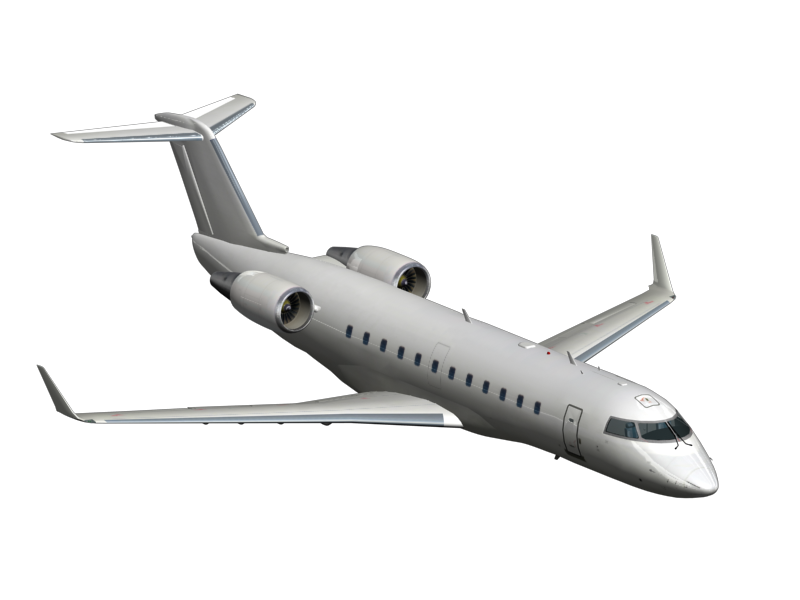
\includegraphics[width=\linewidth]{Figures/Bombardier_CRJ200}
  \end{minipage}%
  \begin{minipage}[b]{0.30\linewidth}
    \centering
    \begin{tabular}[b]{lll}
      \toprule
        \multicolumn{3}{c}{Legend} \\
      \midrule
        A & B & C \\
        0 & 0 & 0 \\
        0 & 1 & 0 \\
        1 & 0 & 0 \\
        1 & 1 & 1 \\
      \bottomrule
    \end{tabular}
    \vspace{5em}
  \end{minipage}
\caption{Figure and table side-by-side.}
\label{fig:side_by_side}
\end{figure}
